For approach-1 and \textit{death}, we got the RMSE comparison results using only CT and CT + Clinical data as described in Table \ref{tab:death_approach_1}. XGBoost performed better than its counterparts with both CT and CT + Clinical Data and exhibited the lowest RMSE. 
\begin{table}[H]
\centering
\begin{tabular}{|l|c|l|}
\hline
\textbf{Model}           & \textbf{RMSE (only CT)} & \textbf{RMSE (CT + Clinical)} \\ \hline
Linear Regression        & 1351.75                 & 1324.57                       \\ \hline
Support Vector Regressor & 1410.32                 & 1381.12                       \\ \hline
XGBoost                  & \textbf{1331.59}                 & \textbf{1314.85}                       \\ \hline
\end{tabular}
\caption{Predicting Death Approach-1:Model Comparison}
\label{tab:death_approach_1}
\end{table}

\begin{figure}[H]
	\def\imgwidth{0.5\linewidth}
% 	\setlength\tabcolsep{2pt}
	\centering
	\begin{tabular}{ccc}
		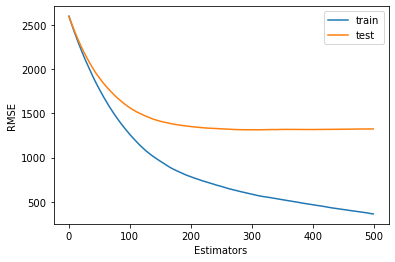
\includegraphics[width=0.3\linewidth]{images/death/a_1_comp_rmse.png} &
		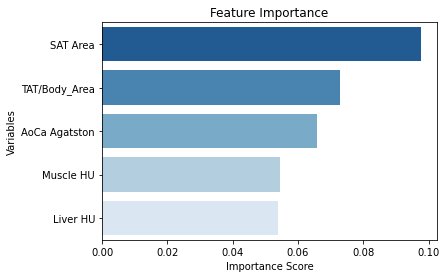
\includegraphics[width=0.3\linewidth]{images/death/a_1_comp_feat_imp.png} &
		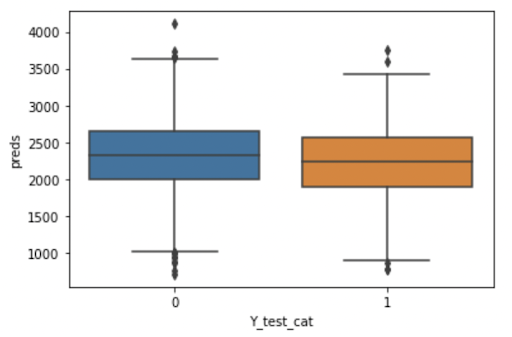
\includegraphics[width=0.3\linewidth]{images/death/a_1_comp_w_test.png} \\
	\end{tabular}
	\caption{XGBoost - Predicting death without recency(approach-1). left = decreasing RMSE with number of iterations, center = feature importance, right = distribution comparison with test-data}
	\label{fig:death_results_a_1}
\end{figure}



For approach-2 and \textit{death}, we got the RMSE comparison results using only CT and CT + Clinical data as described in Table \ref{tab:death_approach_2}. Again, XGBoost performed better than its counterparts with both CT and CT + Clinical Data and exhibited the lowest RMSE. 
\begin{table}[H]
\centering
\begin{tabular}{|l|c|l|}
\hline
\textbf{Model}           & \textbf{RMSE (only CT)} & \textbf{RMSE (CT + Clinical)} \\ \hline
Linear Regression        & 0.235                   & 0.204 (+13.1\%)               \\ \hline
Support Vector Regressor & 0.235                   & 0.243 (-3.4\%)                \\ \hline
XGBoost                  & \textbf{0.232}                   & \textbf{0.212 (+8.6\%)}                \\ \hline
\end{tabular}
\caption{Predicting Death Approach-2:Model Comparison}
\label{tab:death_approach_2}
\end{table}

\begin{figure}[H]
	\def\imgwidth{0.5\linewidth}
% 	\setlength\tabcolsep{2pt}
	\centering
	\begin{tabular}{ccc}
		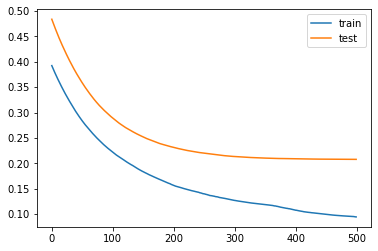
\includegraphics[width=0.3\linewidth]{images/death/a_2_comp_rmse.png} &
		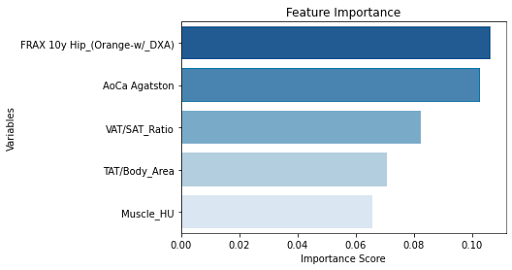
\includegraphics[width=0.3\linewidth]{images/death/a_2_comp_feat_imp.png} &
		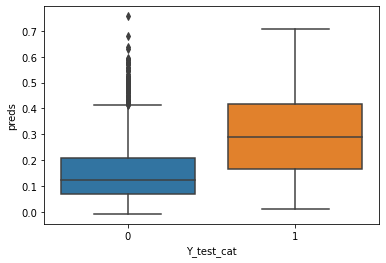
\includegraphics[width=0.3\linewidth]{images/death/a_2_comp_w_test.png} \\
	\end{tabular}
	\caption{XGBoost - Predicting death with recency(approach-2). left = decreasing RMSE with number of iterations, center = feature importance, right = distribution comparison with test-data}
	\label{fig:death_results_a_2}
\end{figure}

We compared the results from both the approaches with the distribution of death, and found out that distribution in approach-1 result is almost same as test-data. However, with approach-2, it is slightly higher(lower because recency is inverse of days). Hence, approach-2 is better.
The approach-1 output SAT Area, TAT/Body Area, AoCa Agatston, Muscle HU, Liver HU as the important features. On the other hand, the approach-2 considers FRAX, AoCa Agatston, VAT/SAT Ratio, TAT/Body Area, Muscle HU. Considering both the approaches, it seems that \textit{AoCa Agatston, TAT/Body Area, Muscle HU} are important features.

\begin{figure}[H]
	\def\imgwidth{0.5\linewidth}
% 	\setlength\tabcolsep{2pt}
	\centering
	\begin{tabular}{cc}
		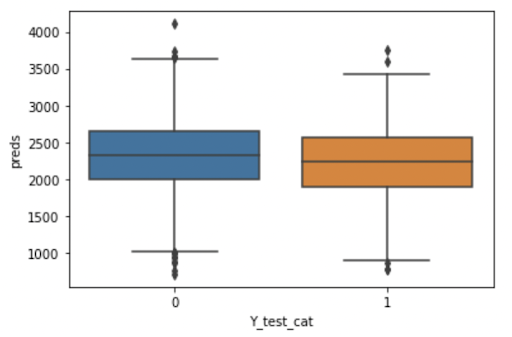
\includegraphics[width=0.4\linewidth]{images/death/a_1_comp_w_test.png} &
		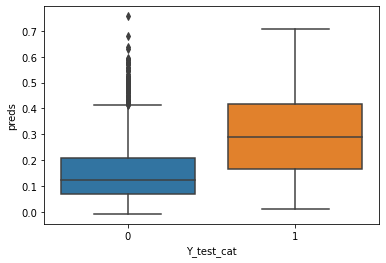
\includegraphics[width=0.4\linewidth]{images/death/a_2_comp_w_test.png} \\
	\end{tabular}
	\caption{Comparison of both the approaches with test data on death distribution. left=approach-1, right=approach-2}
	\label{fig:death_results_dist_comp_with_test_data}
\end{figure}

We continued the same experiments with other clinical outcomes, and found out that \textit{recency} approach is effective in the given dataset.

For approach-2 and \textit{diabetes}, we got the RMSE comparison results using only CT and CT + Clinical data as described in Table \ref{tab:diabetes_approach_2}. Linear Regression performed better than its counterparts with both CT and CT + Clinical Data and exhibited the lowest RMSE. 
\begin{table}[H]
\centering
\begin{tabular}{|l|c|l|}
\hline
\textbf{Model}           & \textbf{RMSE (only CT)} & \textbf{RMSE (CT + Clinical)} \\ \hline
Linear Regression        & \textbf{0.248}                   & \textbf{0.243 (-2\%)}         \\ \hline
Support Vector Regressor & 0.253                   & 0.258 (+1.9\%)                \\ \hline
XGBoost                  & 0.257                   & 0.251 (-2.3\%)                \\ \hline
\end{tabular}
\caption{Predicting Diabetes Approach-2:Model Comparison}
\label{tab:diabetes_approach_2}
\end{table}


For approach-2 and \textit{heart attack}, we got the RMSE comparison results using only CT and CT + Clinical data as described in Table \ref{tab:diabetes_approach_2}. Linear Regression and XGBoost both performed better than Support Vector Regressor with both CT and CT + Clinical Data and exhibited the great improvements. 
\begin{table}[H]
\centering
\begin{tabular}{|l|c|l|}
\hline
\textbf{Model}           & \textbf{RMSE (only CT)} & \textbf{RMSE (CT + Clinical)} \\ \hline
Linear Regression        & 0.223                   & \textbf{0.221 (-0.8\%)}       \\ \hline
Support Vector Regressor & 0.243                   & 0.241 (+0.8\%)                \\ \hline
XGBoost                  & 0.245                   & \textbf{0.230 (-6.1\%)}       \\ \hline
\end{tabular}
\caption{Predicting Heart Attack Approach-2:Model Comparison}
\label{tab:heart_attack_approach_2}
\end{table}